\documentclass[preprint,3p,twocolumn]{elsarticle}
%\documentclass[twocolumn]{elsarticle}
\usepackage[displaymath, mathlines, running]{lineno}
\usepackage{hyperref}
\usepackage{graphicx}
\usepackage{epstopdf}
\usepackage{grffile}
\usepackage{color}


\usepackage[separate-uncertainty = true,
    multi-part-units = single,
    range-phrase = --,
    range-units = single,
    exponent-product = \cdot,
    per-mode = symbol]{siunitx}
\sisetup{
    math-micro = \mu,
    text-micro  = $\mu$
}
\DeclareSIUnit\clight{\text{\ensuremath{c}}}
\DeclareSIUnit\ppm{\text{ppm}}
\DeclareSIUnit\pixel{\text{pixel}}

\DeclareFontEncoding{LS1}{}{}
\DeclareFontSubstitution{LS1}{stix}{m}{n}
\DeclareRobustCommand{\diameter}{%
\text{\usefont{LS1}{stixscr}{m}{n}\symbol{"60}}%
}

\usepackage[fleqn]{amsmath}
\modulolinenumbers[5]

\journal{Journal of \LaTeX\ Templates}

%%%%%%%%%%%%%%%%%%%%%%%
%% Elsevier bibliography styles
%%%%%%%%%%%%%%%%%%%%%%%
%% To change the style, put a % in front of the second line of the current style and
%% remove the % from the second line of the style you would like to use.
%%%%%%%%%%%%%%%%%%%%%%%

%% Numbered
%\bibliographystyle{model1-num-names}

%% Numbered without titles
%\bibliographystyle{model1a-num-names}

%% Harvard
%\bibliographystyle{model2-names.bst}\biboptions{authoryear}

%% Vancouver numbered
%\usepackage{numcompress}\bibliographystyle{model3-num-names}

%% Vancouver name/year
%\usepackage{numcompress}\bibliographystyle{model4-names}\biboptions{authoryear}

%% APA style
%\bibliographystyle{model5-names}\biboptions{authoryear}

%% AMA style
%\usepackage{numcompress}\bibliographystyle{model6-num-names}

%% `Elsevier LaTeX' style
\bibliographystyle{elsarticle-num}
%%%%%%%%%%%%%%%%%%%%%%%

\begin{document}

\begin{frontmatter}

\title{ Development of a Microchannel Plate Based Beam Profile Monitor for Re-accelerated Muon Beam}
%\tnotetext[mytitlenote]{Fully documented templates are available in the elsarticle package on \href{http://www.ctan.org/tex-archive/macros/latex/contrib/elsarticle}{CTAN}.}

%% Group authors per affiliation:
%\author{B.Kim\fnref{myfootnote}}
%\address{Seoul National University}
%\fntext[myfootnote]{Since 1880.}

%% or include affiliations in footnotes:
\author[mymainaddress,mymainaddress1]{Bongho~Kim}
\ead{bhokim@hep1.snu.ac.kr}
%\ead[url]{www.elsevier.com}
\author[mymainaddress,mymainaddress1]{Sunghan~Bae}
\ead{bco2000@snu.ac.kr}
\author[mymainaddress,mymainaddress1]{Hyunsuk~Choi}
\author[mymainaddress,mymainaddress1]{Seonho~Choi}
\author[fifthaddress,fifthaddress1]{Naritoshi~Kawamura}
\author[secondaddress]{Ryo~Kitamura}
\author[mymainaddress,mymainaddress1]{Ho~San~Ko}
\author[seventhaddress]{Yasuhiro~Kondo}
\author[thirdaddress]{Tsutomu~Mibe}
\author[thirdaddress]{Masashi~Otani}
\author[fourthaddress,fourthaddress1,pulkovo]{Georgiy~P.~Razuvaev}
\author[sixthaddress]{Eunil~Won}
%\author[mysecondaryaddress]{Global Customer Service\corref{mycorrespondingauthor}}
%\cortext[mycorrespondingauthor]{Corresponding author}
 %support@elsevier.com}
\address[mymainaddress]{Department of Physics and Astronomy, Seoul National University, Seoul, 08826, Korea}
\address[mymainaddress1]{Institute for Nuclear and Particle Astrophysics, Seoul National University, Seoul, 08826, Korea}
\address[secondaddress]{Department of Physics, University of Tokyo, Tokyo 113-0033, Japan}
\address[thirdaddress]{High Energy Accelerator Research Organization (KEK), Tsukuba 305-0801, Japan}
\address[fourthaddress]{Budker Institute of Nuclear Physics SB RAS, Novosibirsk 630090, Russia}
\address[fourthaddress1]{Novosibirsk State University, Novosibirsk 630090, Russia}
\address[pulkovo]{Pulkovo Observatory, St. Petersburg, 196140, Russia}
\address[fifthaddress]{Muon Sci. Lab., Institute of Materials Structure Science, High Accelerator Research Organization, Tsukuba, 305-0801, Japan}
\address[fifthaddress1]{Muon Sci. Sec., Materials and Life Science Facility, J-PARC, Tokai, 319-1195, Japan}
\address[sixthaddress]{Department of Physics, Korea University, Seoul, 02841, Korea}
\address[seventhaddress]{Japan Atomic Energy Agency (JAEA), Tokai, 319-1195, Japan}
%\address[mysecondaryaddress]{360 Park Avenue South, New York}

\begin{abstract}
  A beam profile monitor (BPM) based on a microchannel plate has
  been developed for \iffalse ultracold\fi muon beams with low transverse momentum for the measurement of
  the muon anomalous magnetic moment and electric dipole moment at
  high precision, with capability of diagnosing muon beams of kinetic
  energy range from a few \si{keV} to \SI{4}{MeV}.  The
  performance of the BPM has been evaluated using a surface muon
  beam at J-PARC and additionally with an ultraviolet (UV) light source.  It has
  been confirmed that the BPM has a dynamic range from a few to
  $10^4$ muons per bunch without saturation.  The spatial resolution of
  the BPM has been estimated to be less than \SI{0.30}{\mm}.  A
  partial discrimination of positrons from muons has
  been achieved under discrete particle conditions.

\end{abstract}

\begin{keyword}
%Ultracold muon
Low emittance muon beam \sep Beam diagnostics \sep Microchannel plate \sep Beam profile
%\texttt{elsarticle.cls}\sep \LaTeX\sep Elsevier \sep template
%\MSC[2010] 00-01\sep  99-00
\end{keyword}

\end{frontmatter}

\linenumbers

% GMM General comments:
%
% The term "ultracold" is not appropriate for particles or atoms
% above a few times 1.e-7 K, while these muons are 300 K. See
%
% https://en.wikipedia.org/wiki/Ultracold_atom 
%
% I suggest to replace "ultracold" with "thermal".
%
% The references should be checked carefully and put into a
% consistent format as required by the journal. In particular the
% references [14] and [15] should have page and year.


\section{Introduction}

The J-PARC muon $g-2$/EDM experiment \cite{E34} aims to measure
the muon anomalous magnetic moment ($a_{\mu} = (g_{\mu}-2)/2$) and the muon electric
dipole moment (EDM) with high precision.  A new beam line for
muons (H-line)~\cite{h-line} is under development.  The
experiment requires a muon beam with small transverse emittance
that is obtained by re-accelerating ultraslow muons.  The
ultraslow muons are produced from ionization of muonium
($\mu^{+}e^{-}$) at thermal
energy with lasers.  Muonium is produced by stopping a surface muon
beam in a muonium production target~\cite{muonium}.  This muon
beam with low transverse momentum will be re-accelerated to the momentum value of
\SI{300}{\MeV\per\clight} \cite{IH} while minimizing the increase
of the transverse momentum ($\sigma_{pT}/p = 10^{-5}$).  The
accelerated muon beam is injected to the storage area under
\SI{3}{\tesla} magnetic field without electric
focusing~\cite{injection}.  The experiment measures $g-2$ with a
precision of \SI{0.1}{\ppm} and the EDM with a sensitivity to
\SI{e-21}{\elementarycharge \cdot \cm}.  Proper beam diagnostics
are required for the development of this new muon beam.

In contrast to other surface muon monitors~\cite{muon_bpm1,
muon_bpm3}, our BPM is designed to measure a beam profile and
relative intensity for each bunch simultaneously from low
intensity (a few muons per bunch) to high intensity in the kinetic energy
range from a few \si{keV} to \SI{4}{\MeV}.  A BPM based on
a Micro-Channel Plate (MCP) has been developed to obtain necessary
gain and efficiency to measure a low intensity beam.  There have
been several experiments that have used detectors based on an MCP
assembly to work with beams of muons, neutrons, ions, atoms and
positronium~\cite{muon_bpm2, neutron, Ps}.  Unlike
other beams, muons are stopped in the MCP due to a short penetration depth
and decay to positrons plus muon antineutrinos and electron
neutrinos by the weak interaction. These positrons give signals in
the BPM via penetration of the MCP channels.  Understanding and
subtracting this positron background from the muon signal is one
of the challenges in measuring a precise beam profile.

In this paper, we present the design and results of tests using
the surface muon beam and the UV light source.  The responses of
muon and positron signals and the signal linearity were measured
by the surface
muon beam.  The spatial resolution was measured by a UV light
with a semicircular hole collimator.


\section{BPM design and specification}

Our BPM is designed to characterize a muon beam with sub-millimeter
resolution for a $\sim$\SI{10}{\mm} beam spot size for the kinetic energy
range from a few \si{\keV} to \SI{4}{\MeV} corresponding to the low $\beta$ section
of the muon LINAC \cite{IH}.  The BPM aims to measure a muon
intensity from a few muons to \num{e5} muons per bunch at a
repetition rate of \SI{25}{\hertz}.

As shown in Fig.~\ref{fig:BPM_scheme}, the BPM consists of two
stages of MCP, one stage of a phosphor screen and a charge-coupled device (CCD) camera.
High efficiency for \si{\keV} order atomic and ion beams has been
observed in several experiments \cite{MCP_efficiency,
MCP_efficiency1}. Similar high efficiency for a low energy muon
beam is expected.

\begin{figure}
\begin{center}
\vspace{-2.5cm}
%\begin{minipage}[t]{70mm}
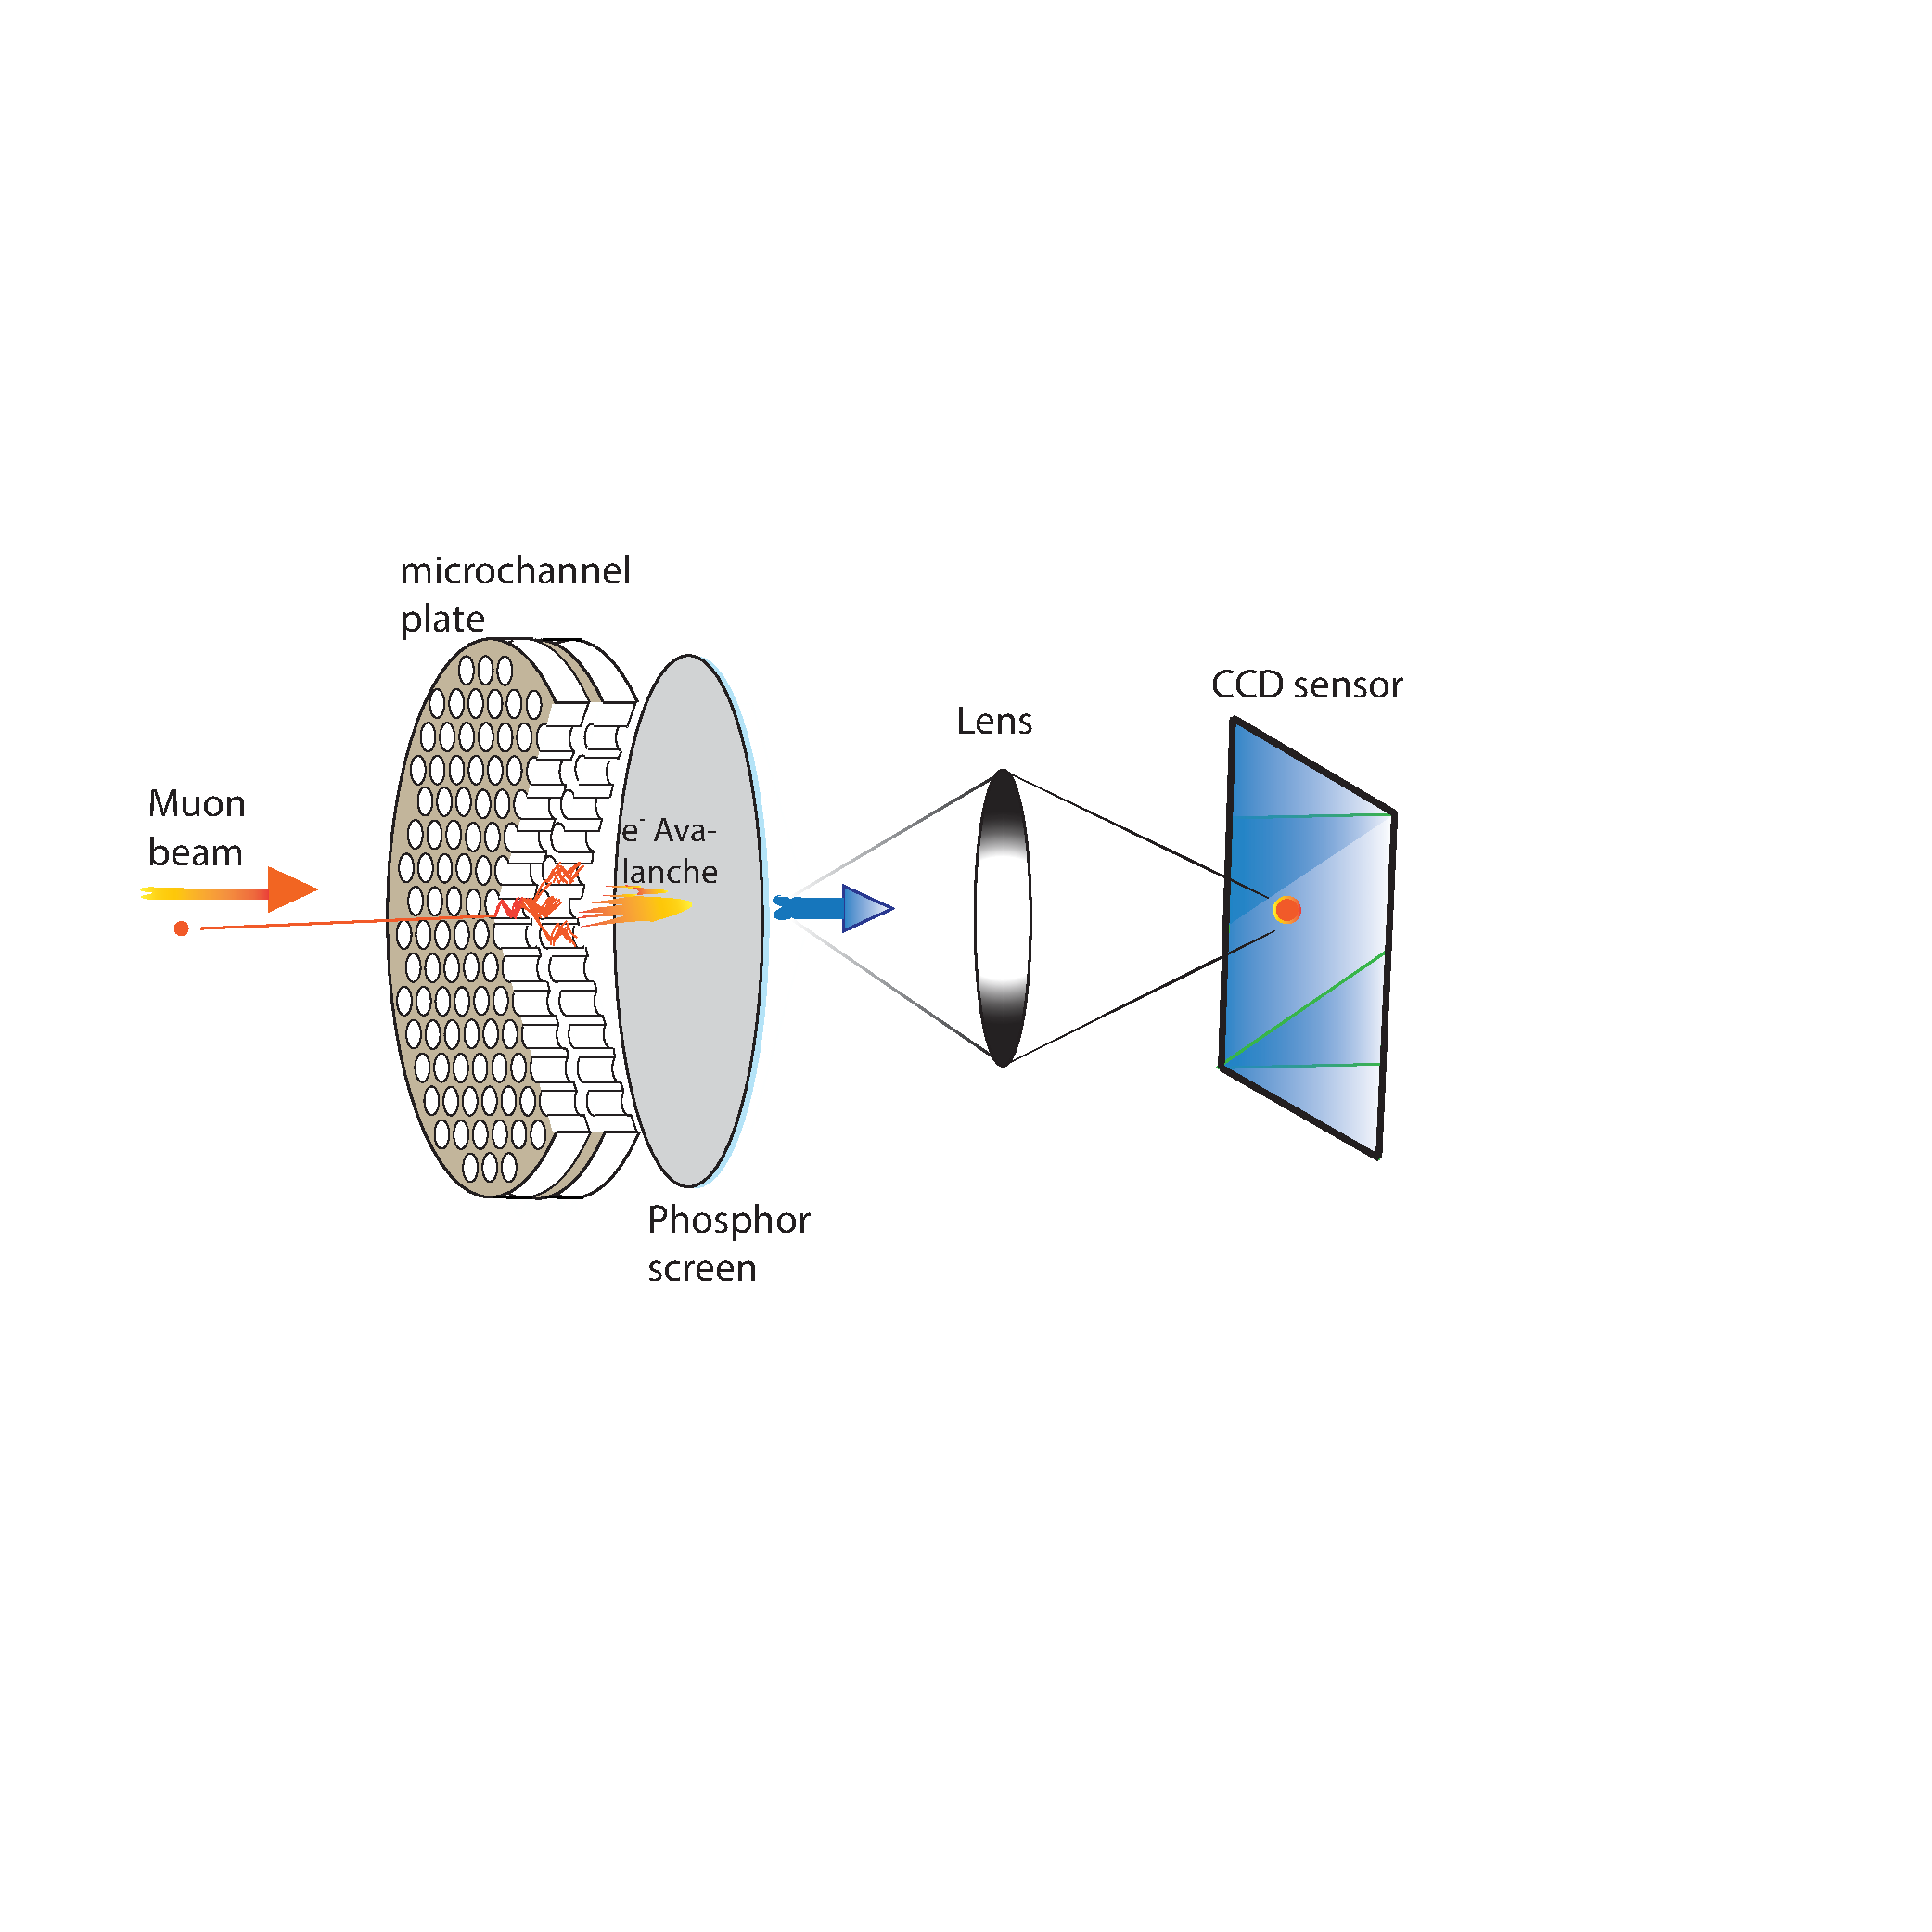
\includegraphics[width=0.6\textwidth, height=0.6\textwidth]{figure/bpm_v3.pdf}
\vspace{-3cm}
\caption{A schematic view of the MCP based BPM.}
\vspace{-0.5cm}
%\end{minipage}
\label{fig:BPM_scheme}
\end{center} \end{figure}

The MCP assembly (Hamamatsu F2225-21P) has two stages of chevron
type MCPs with an effective area corresponding to a diameter
of $\diameter = \SI{40}{\mm}$ and
gain of \numrange{e6}{e7} plus a phosphor screen (P47). The
light output from the phosphor screen is transmitted through a
glass viewport (7056 borosilicate) and then captured by the
cooled CCD camera (PCO PCO1600: $800 \times 600$ pixels with
combined $2 \times 2$ binning mode) with lens (Zeiss
Distagon 2/28 ZF.2).  In order to block the electron background,
negative potential (\SI{-1.9}{\kilo\volt}) is applied in the MCP
front surface.  The MCP back surface is connected to a ground
after an electric circuit to read out the electric signal of the
MCP.  Positive potential (\SI{3.9}{\kilo\volt}) is applied to the
phosphor screen.

The exposure time of the CCD camera is set to \SI{0.5}{\micro\s} to
reject positrons from the muon decay
($\tau = \SI{2.2}{\micro\s}$ \cite{muon_pdg}).  The P47 phosphor
material (Y$_2$SiO$_5$:Ce) is chosen to have a short decay time
($\tau_{\SI{10}{\percent}} = \SI{0.11}{\micro\s}$) compared to
the exposure time to enable this discrimination method.

The MCP assembly is installed in the middle of a cylindrical
vacuum chamber constructed from stainless steel.  The MCP
assembly and the CCD camera are aligned in the cylindrical axis.
The vacuum chamber has a thin mylar film (\SI{0.1}{mm}) window with $\diameter=\SI{100}{\mm}$ in
% GMM add window diameter here?
a flange in front of the MCP assembly for beam transmission.
Another mylar film window is installed in a side port for
positron transmission.  There is a viewport in a flange behind the MCP
assembly.

\section{Experiment with muon beam}

\subsection{Experimental setup} 

A schematic view of the experimental setup for the surface muon
beam test
is shown in Fig. \ref{fig:simulation}.  The J-PARC
muon facility provides surface muon ($\mu^{+}$) beam in single pulse mode
to the Material and Life Science Experimental Facility (MLF)
D-line D2 area with \SI{100}{\nano\s} beam width,
\SI{4}{\MeV} kinetic energy, \SI{25}{\hertz} repetition
rate, and the intensity of a few $10^{6~}\mu^{+}$\SI{}{/\s}~\cite{muon_bpm3, D-line1}.  The beam intensity was adjusted by
slits in the beamline.  The beam size and intensity were further
adjusted by installing one of a set of lead collimators with
$\diameter=\SI{10}{\mm}$, $\SI{20}{\mm}$ or $\SI{40}{\mm}$ hole
between the exit window of the beam line and the BPM
% The intensity was adjusted with slits and collimator. What was
% the range of muon intensity and of beam positron intensity?
% The specific numbers for the selected experimental
% arrangement(s) should be specified when displaying the data in
% the next sections as well.
vacuum chamber.  The MCP assembly was installed inside the BPM
vacuum chamber which was separated from the beam line as an
independent vacuum system.

The number of muons on the BPM was measured from decay positrons.
A fraction of the decay positrons from muons stopped in the
MCP volume go through the mylar film in the side port of the BPM
chamber and give signals to the positron counter. %The number ratio of such positrons and %muons on the BPM is
%determined by the simulation as described in data analysis part.
% GMM this is my understanding, but please make sure it is correct
The positron
counter consists of two plastic scintillators with corresponding
light guides and PMTs.  The positron counter was shielded by lead
blocks to suppress decay positrons from directions other than from
the MCP.  A lead collimator with a
$\diameter = \SI{30}{\mm}$ hole was used to provide a direct view
of the MCP from the positron counter.

\begin{figure}[tb]
{\setlength{\belowdisplayskip}{0pt}
\begin{minipage}[t]{60mm}
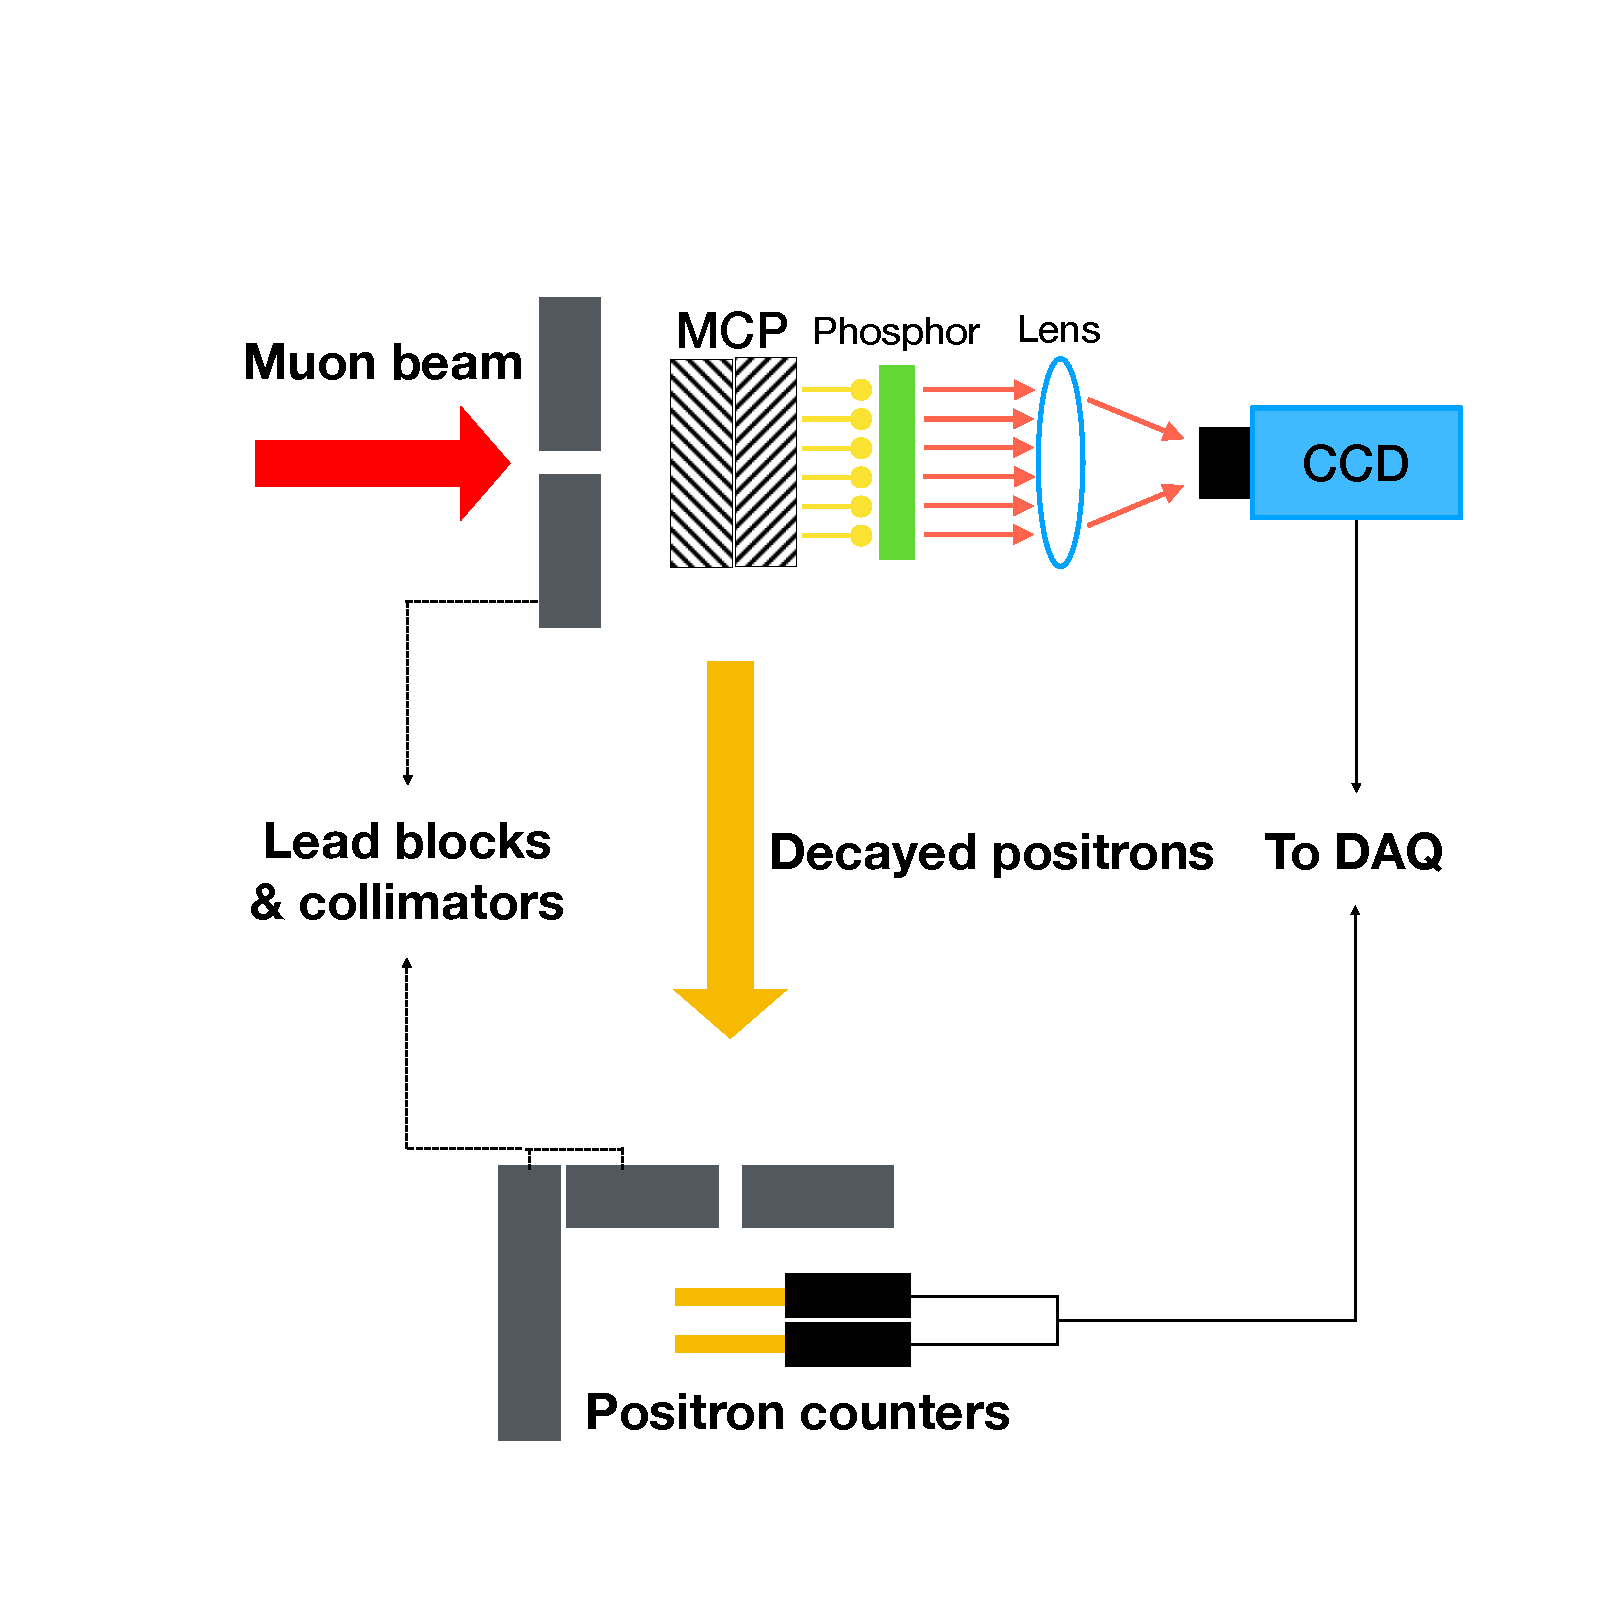
\includegraphics[width=1.25\textwidth, height=1.25\textwidth]{figure/BPM_schematic_2.pdf}
\end{minipage}
}
\caption{Setup for the test with muon beam at the J-PARC MLF D-line D2
  area.}
\vspace{-0.4cm}
\label{fig:simulation}
\end{figure}

\subsection{Data taking} 

Two dimensional pictures were taken by the CCD camera with
\SI{500}{\nano\s} exposure time.  The arrival time of the muon
beam was measured by the electronic signal of the MCP. This timing
information was used to set the proper timing for triggering the
CCD exposure. The exposure at the arrival time of the muon beam ($t_{delay} = \SI{0}{\micro\s}$) was set by matching the center of exposure time window with the measured arrival time. The waveform data for the positron counter was
taken for a $\SI{10}{\micro\s}$ period in coincidence with the
muon beam pulse.

Data with a few muons per pulse were taken to understand the
properties of a single muon signal.  Data with higher
intensities were then taken by changing the sizes of the slit in
the beam line and the collimator.  Another set of data was
taken with different trigger timing for the CCD camera to understand
positron signals in the BPM.  Typical CCD images taken at
different intensities are displayed in
Fig.~\ref{fig:single_cluster}. A raw picture (Fig.~\ref{fig:single_cluster}a) and
the accumulation of 1000 pictures in a two dimensional histogram (Fig.~\ref{fig:single_cluster}b) were taken
with the high intensity muon beam. Low intensity pictures are
shown for camera exposure at the beam arrival (Fig.~\ref{fig:single_cluster}c) and for delayed camera exposure from the beam arrival
by $\SI{2}{\micro\s}$ (Fig.~\ref{fig:single_cluster}d).
% GMM It would be better to describe the subfigures in the same
% order as in the caption, to avoid confusion. Also letters for
% labels would help. Is it correct to conclude that bottom left
% corresponds to 5 muons? If so, it would be better not to let
% the reader make this assumption on his/her own.

\begin{figure}[tbp]
	\centering
	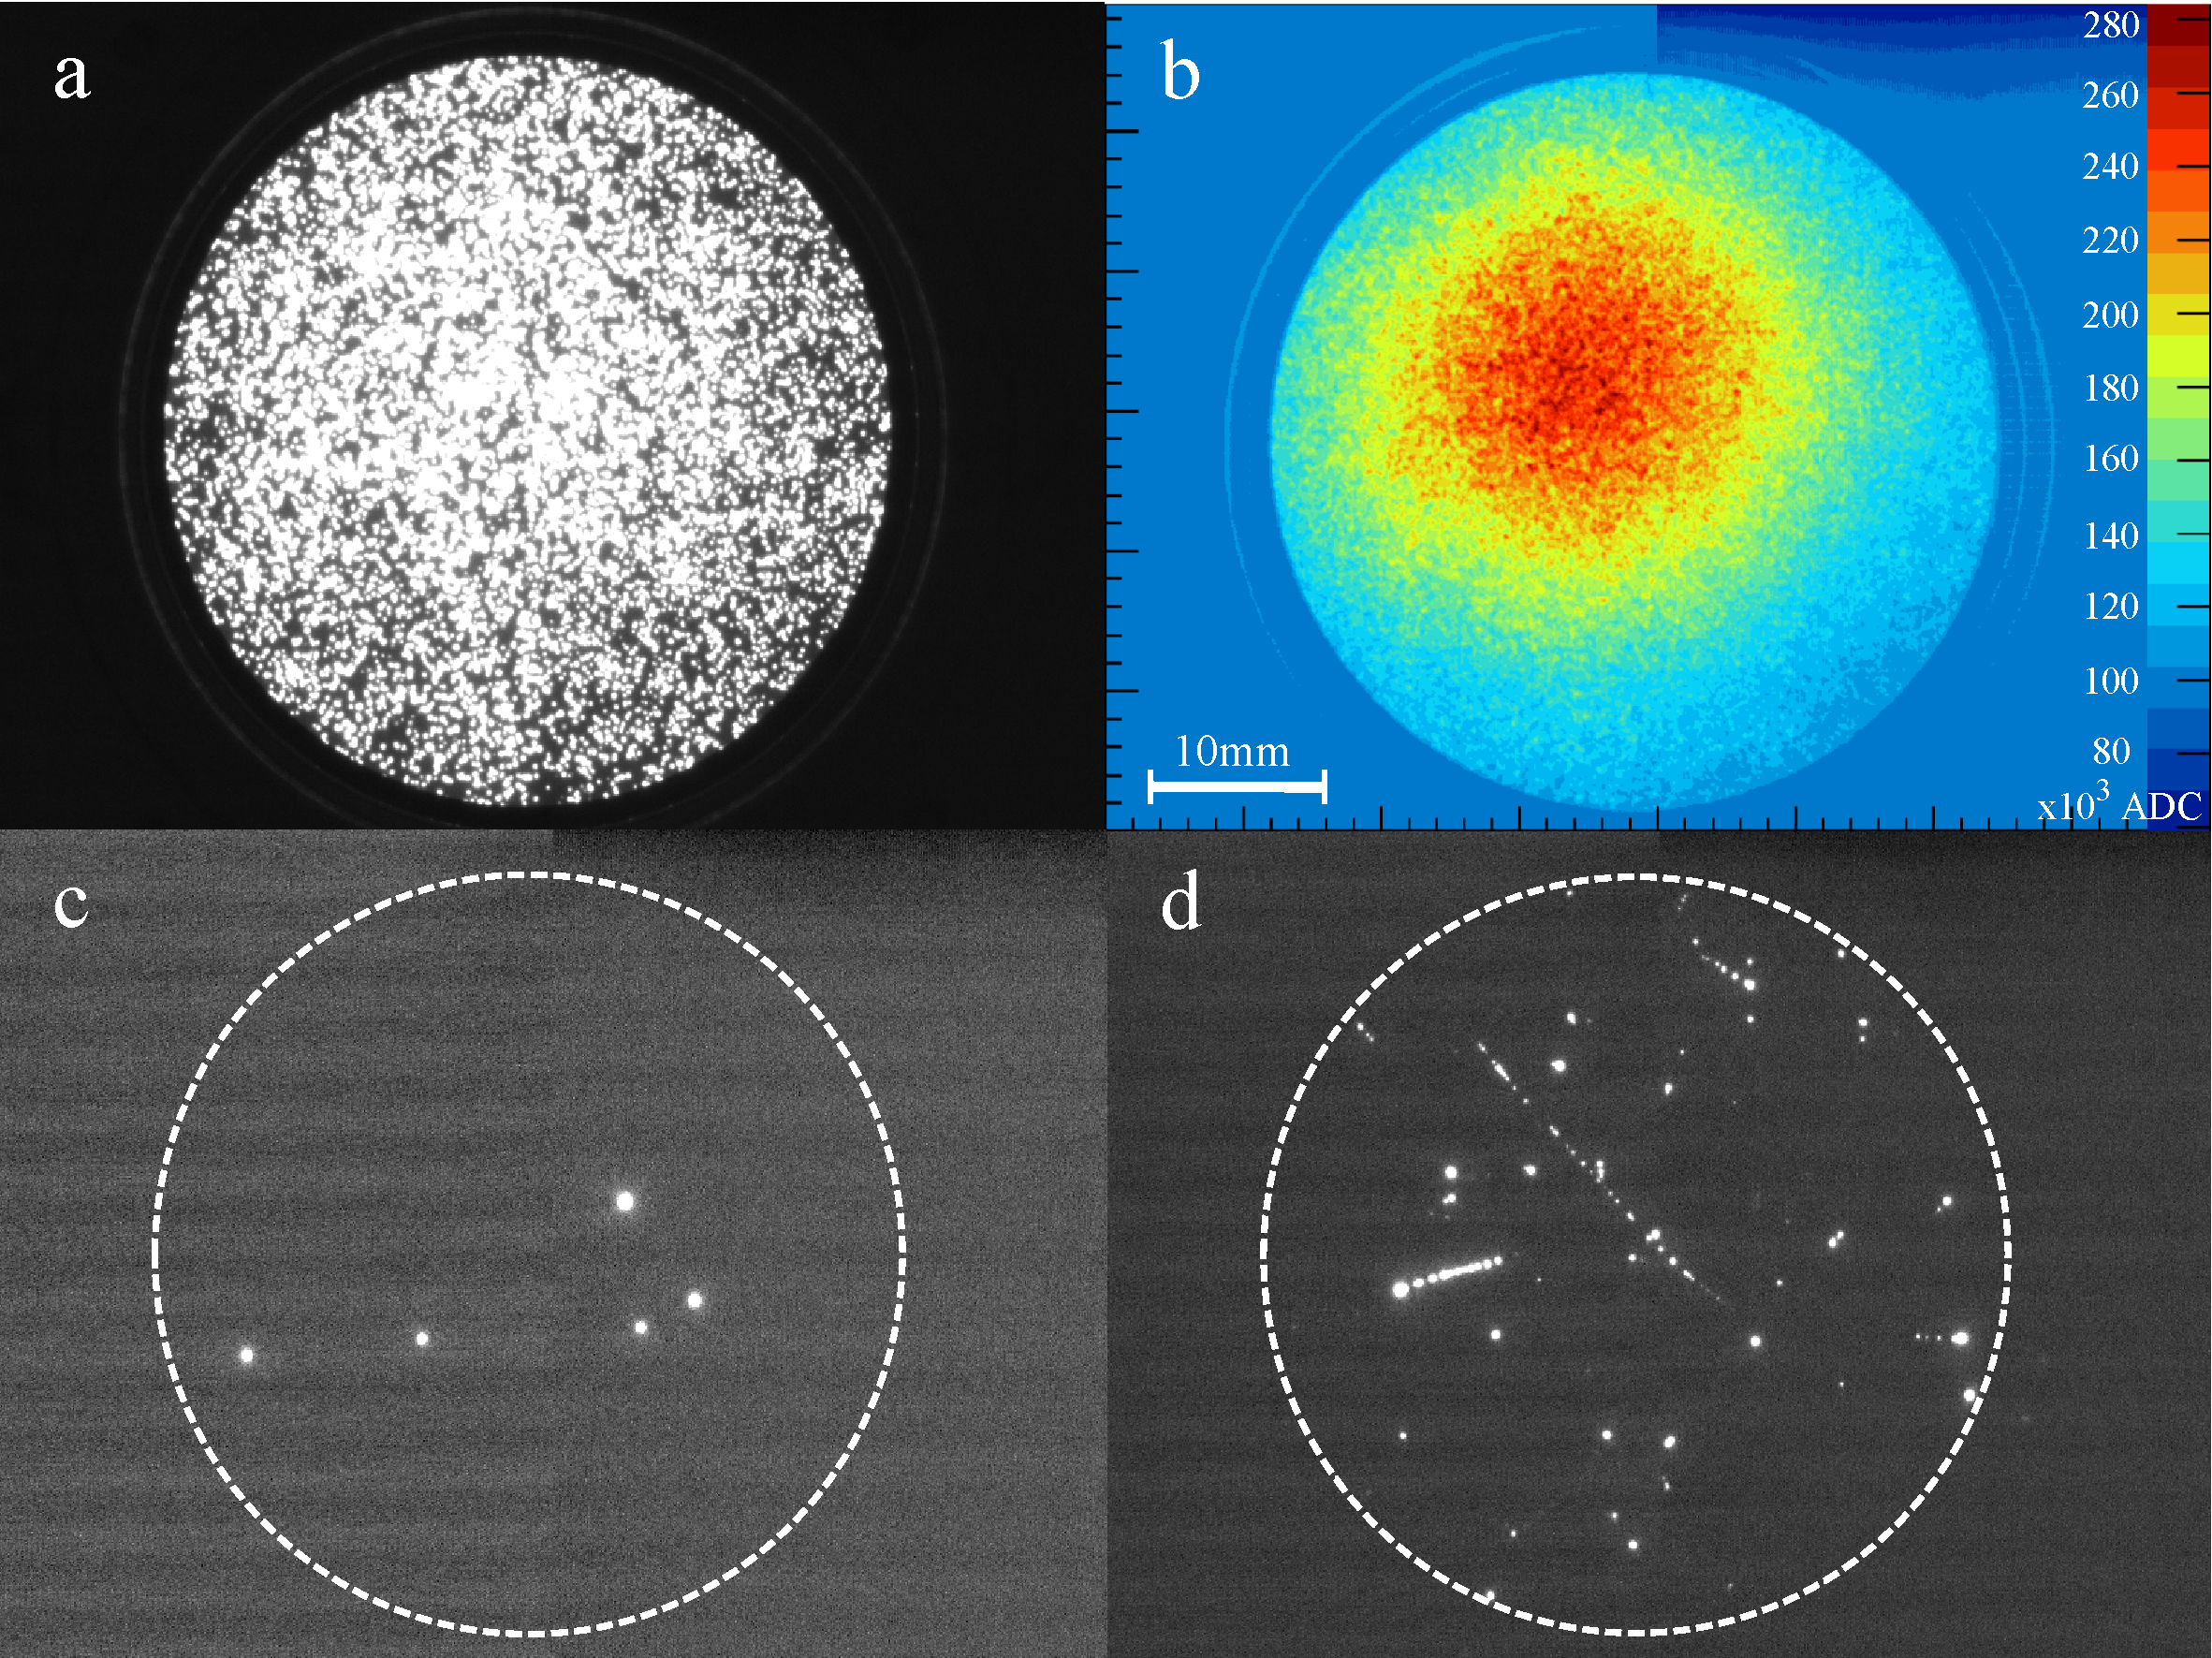
\includegraphics[width=\columnwidth]{figure/fig3_v3_number.pdf}
	\caption{Typical CCD images taken with muon beam. (a) 
		Single picture at high intensity beam. (b)
		Accumulation of 1,000 pictures at high intensity beam. (c) Single picture
		with low intensity beam. (d)
		Single picture of $\SI{2}{\micro\s}$ delayed trigger timing from beam arrival.
        The pixels with higher ADC counts are in white. Dashed lines are artificial drawing of MCP boundary.           }
	\vspace{-0.4cm}
	\label{fig:single_cluster}
\end{figure}
% GMM It might be more clear with labels on the 4 pictures, a),
% b), c) d). Top right does not specify whether dark or light
% color represents exposure. For top left, I have to assume that
% red is higher exposure. Is there a color code for the 2-d
% histogram? Is it a linear or logarithmic display?

% S.Bae: I changed the figure, captions and the text from line 326 in tex. 

\subsection{Data analysis}

As shown in Fig.~\ref{fig:single_cluster}c, visible identification of isolated signals at low intensity is achievable.
%signals are distinguishable from the CCD noise. %by the signal
%shape being a two dimensional sharp Gaussian distribution with
%additional broad tail distribution.
% GMM Fig. 3 does not show a Gaussian distribution or a broad
% tail. What am I missing? I can't understand what you refer to,
% so I can't come to the same conclusion.
%
% S.Bae: I skipped that part in the text. If we need to mention the shape of signal, we need a discussion.
To distinguish the signals from
CCD noise, a cluster is defined for single signal selection. A
single cluster region for each signal is defined as $9 \times 9$
CCD pixels in which a pixel with maximum ADC counts in each signal is centered. This
region is about 5 times of root mean square (RMS) width (1.6
pixel) of a single muon signal (Fig.~\ref{fig:positron_width}). 
% GMM There is no evidence for this claim of RMS for a single
% muon signal. Do you need another figure to show this? Did you
% consider a 9x9 2-d histogram of a large number (e.g. 1000) of
% single muon signals, where the middle channel of the 9x9 array
% corresponds to the pixel with the maximum count for each of the
% single muon signals. With some care (integrating the function
% over the square bin in the fit function definition), a 2-d
% multiple Gaussian with 2 parameters (peak normalization, radial
% width) for each of the multiple Gaussians, plus one more
% parameter for a flat background, could be fit to the 9x9 array,
% also demonstrating consistency with the claimed background and
% showing what you mean by "broad tail distribution".
%The scale of a pixel in the
%picture is determined as \SI{0.08}{\mm \per \pixel} considering
%the size of the MCP active area.
The scale of a pixel in the
picture is determined as \SI{0.08}{\mm \per \pixel} by correlating
the diameter of the MCP active area and its image in the picture.
%In the data, the 40 mm MCP diameter corresponds to 500 pixels, resulting in a scale of 0.08 mm/pixel.
% GMM Do you really mean 0.08 mm/pixel _in the picture_ (i.e., on
% the paper)? If so, be aware that the display of your paper may
% not be to the same scale as you assume when you state 0.08
% mm/pixel, e.g., if someone is reading this online or in a pdf.
% But maybe you mean the scale of the CCD image itself, in (mm at
% the MCP)/(pixels in the CCD). It is better to stay with a
% physical size such as the MCP diameter of 40 mm and the number
% of mm/pixel for that size, and then rely on the scale you have
% in the top left diagram. To make it clear, you could say, " The
% 40 mm MCP diameter corresponds to XXX pixels, resulting in a
% scale of YYY mm/pixel." where YYY = 40/XXX.
%
% S.Bae: I changed it as B.Kim said and put the sentence below.

Each cluster is identified by detecting $3 \times 3$ pixels with
ADC counts above thresholds determined by the CCD noise
fluctuation in RMS value, averaged over pixels, (\SI{8.7}{ADC{~}counts/\pixel}) from each offset ADC counts in each pixel. The properties of single
clusters are studied with this selection criterion.
%Each cluster is identified by detecting $3 \times 3$ pixels which satisfy that
%ADC value in each pixel is larger than mean CCD noise of corresponding pixel by thresholds %determined from the noise fluctuation ($\sigma=$\SI{8.7}{ADC}) which is averaged over all %pixels. The properties of single
%clusters are studied with this selection criterion. 

% GMM This is not clear to me. I suggest to add more detail. Does
% 8.7 ADC mean 8.7 channels of the ADC for each pixel? Is that
% the rms deviation from the mean, or from zero, of the noise as
% measured with no muon beam? Is this per channel or per 3x3
% cluster? The number should be proportional to a gate width,
% presumably the 500 ns exposure time, but that should be
% confirmed in this paragraph. It is not clear whether the
% threshold is just 1 sigma above the mean noise level, or
% several sigma; if it is the latter, how many sigma?
%
% S.Bae : I modified this part to be more clear.
The distribution of the cluster ADC sum is displayed in
Fig.~\ref{fig:BPM_int}.  The ADC sum distribution shows an
isolated peak for exposure to muons, with no corresponding peak
for delayed exposure
($t_{delay} =$ either$~2~$or$~\SI{3}{\micro\s}$).
% GMM Does this mean either 2 or 3 mus delay, each with 500 ns
% width, and that both look the same? Or is it just one delay, a
% window between 2 and 3? The notation is not clear. This is also
% true of the label on the figure.

\begin{figure}[tbp]
	\centering
	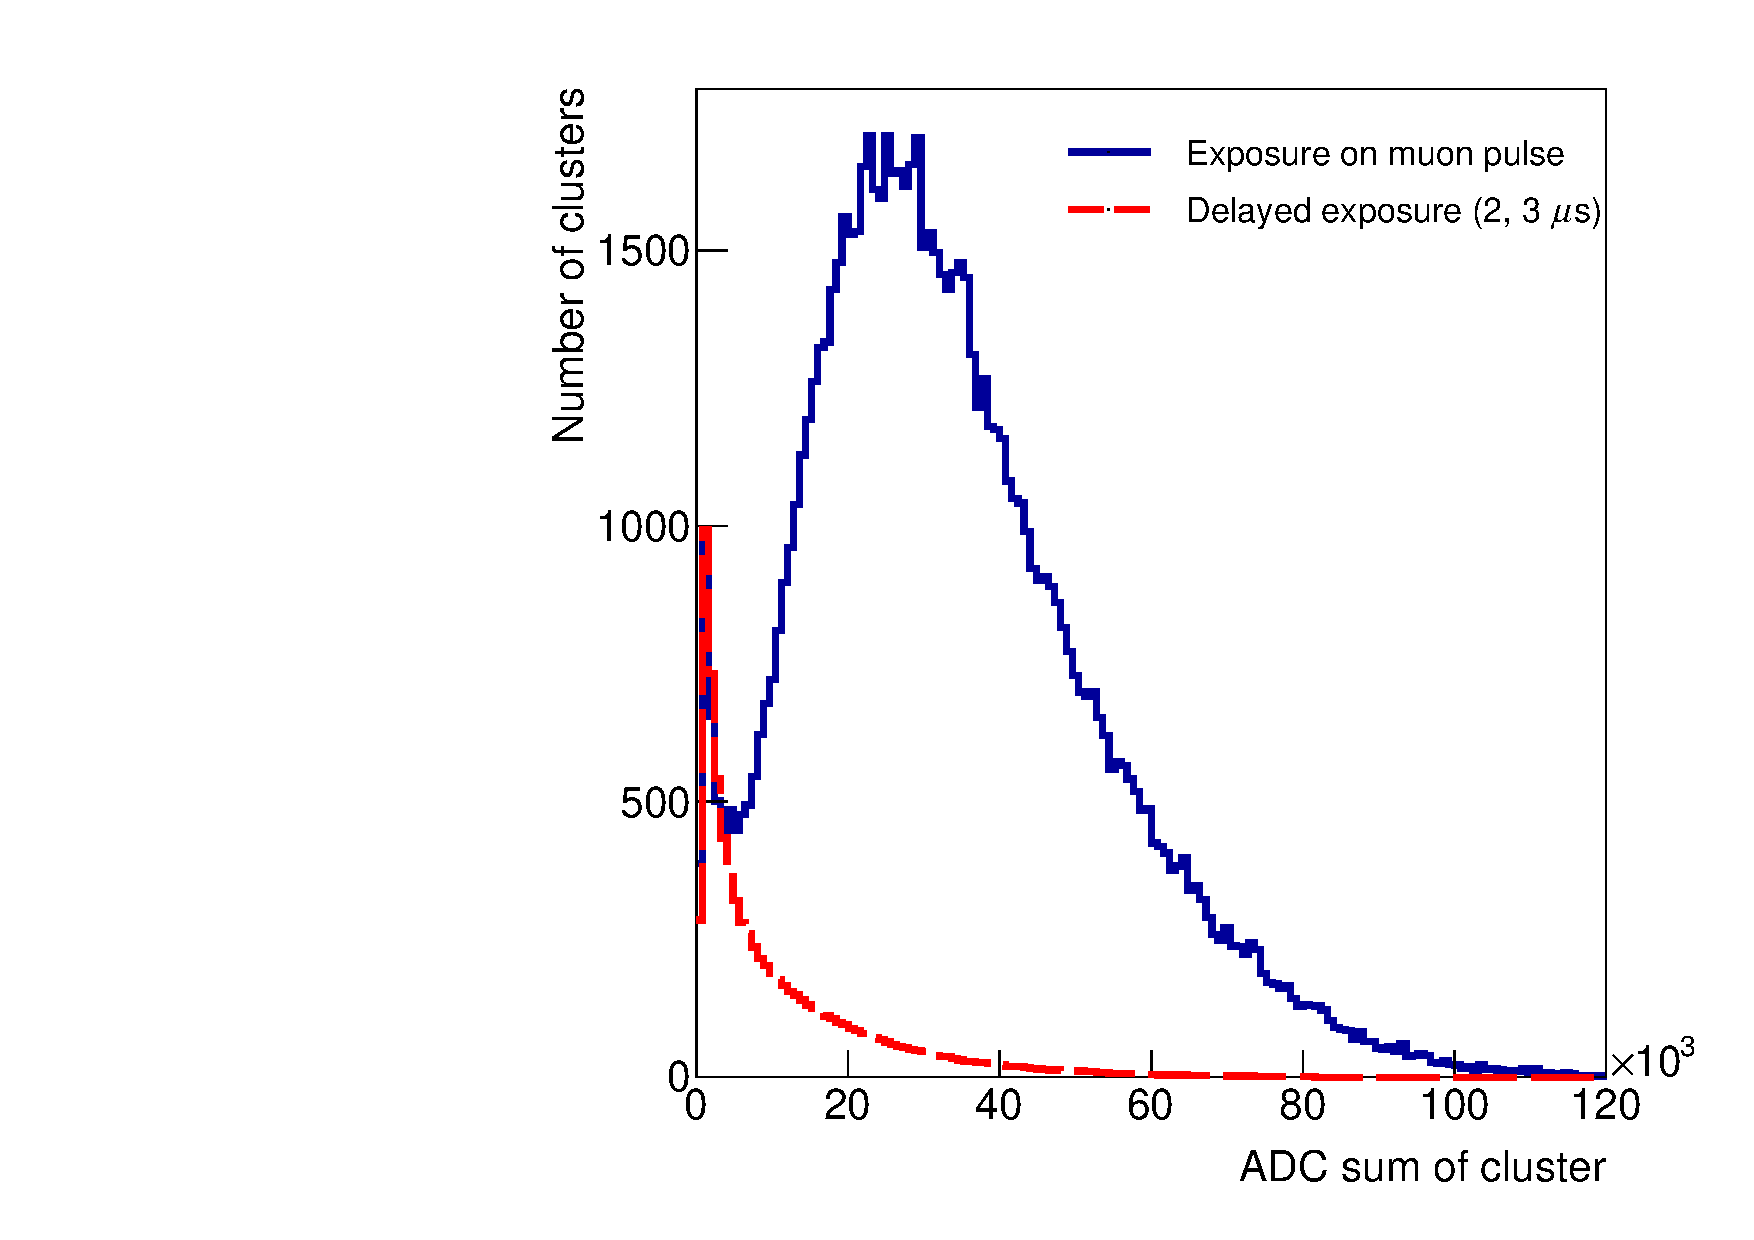
\includegraphics[width=\columnwidth]{figure/Integ_legend_v2.pdf}
	\caption{Cluster ADC sum in $9\times9$ pixels for the
          exposure on muon pulse (solid) and the delayed exposure
          (dashed).  The normalization is done for delayed exposure histogram
          by matching the first peak height to that of exposure on muon pulse histogram.}
	\vspace{-0.2cm}
	\label{fig:BPM_int}
\end{figure}
% GMM The normalization procedure is not explained clearly. What
% is matched? Total exposure time (window times events)? Counts
% in the earliest channel?
%
% S.Bae: More detail is included.

A positron signal pixel distribution can have a non-circular shape or even several
peaks over the signal region because it can penetrate the MCP in
any direction, since decay positrons are generated within the MCP
with momenta in all directions.  
To parametrize the signal
width, the minimum RMS width and the maximum RMS width of the
clusters are calculated by counting pixels. %The
% Calculated how? By a fit? Or by counting pixels?
%maximum width distribution is shown in
%Fig.~\ref{fig:positron_width}.
% GMM This text implies that an ellipse is fitted to each signal
% distribution. If that is true, it should be stated explicitly
% and briefly discussed in the text, and if not, it should be
% re-worded. Since the distributions are narrow for muons and
% presumably for perpendicular decay positrons, the direction of
% the x-y pixel arrangement compared with the transverse positron
% direction should be expected to be important in the width
% distribution, as the pixel sizes (and resolutions in terms of
% pixels) are different for axes other than x and y. This could
% be confirmed or otherwise by checking width distributions for
% large (near 45 degrees) vs small (near 0 or 90 degrees)
% absolute axis rotation values.

For data in the muon beam time window, the maximum and minimum of
the width distribution
are almost the same, except for
a small tail in the maximum width distribution. This is because
the incident muon has mainly longitudinal momentum and makes a
symmetric signal.  
% GMM From previous experience, I believe the small tail in the
% maximum is from muons which decay within the 500 ns muon time
% window, such that the positron energy loss is included with the
% muon signal. If that is true, the maximum width cut would
% remove muons that decay in this time range into positrons with
% transverse momentum. Be aware of this as a possible
% time-position correlation bias in event selection.
For the delayed exposure data
% GMM Again, the notation is not clear below.
($t_{delay} =$ either$~2~$or$~\SI{3}{\micro\s}$), the minimum width distribution is
similar to that of the muon signal, but the maximum width
distribution shows an excess at large RMS width value as shown in Fig.~\ref{fig:positron_width}. Under the maximum
RMS width cut ($\Gamma_{max} < \SI{0.15}{\mm}$),
\SI{57}{\percent} of the clusters in the delayed exposure
survived while \SI{94}{\percent} of the clusters in the muon
pulse exposure survived.

\begin{figure}[tbp]
	\centering
	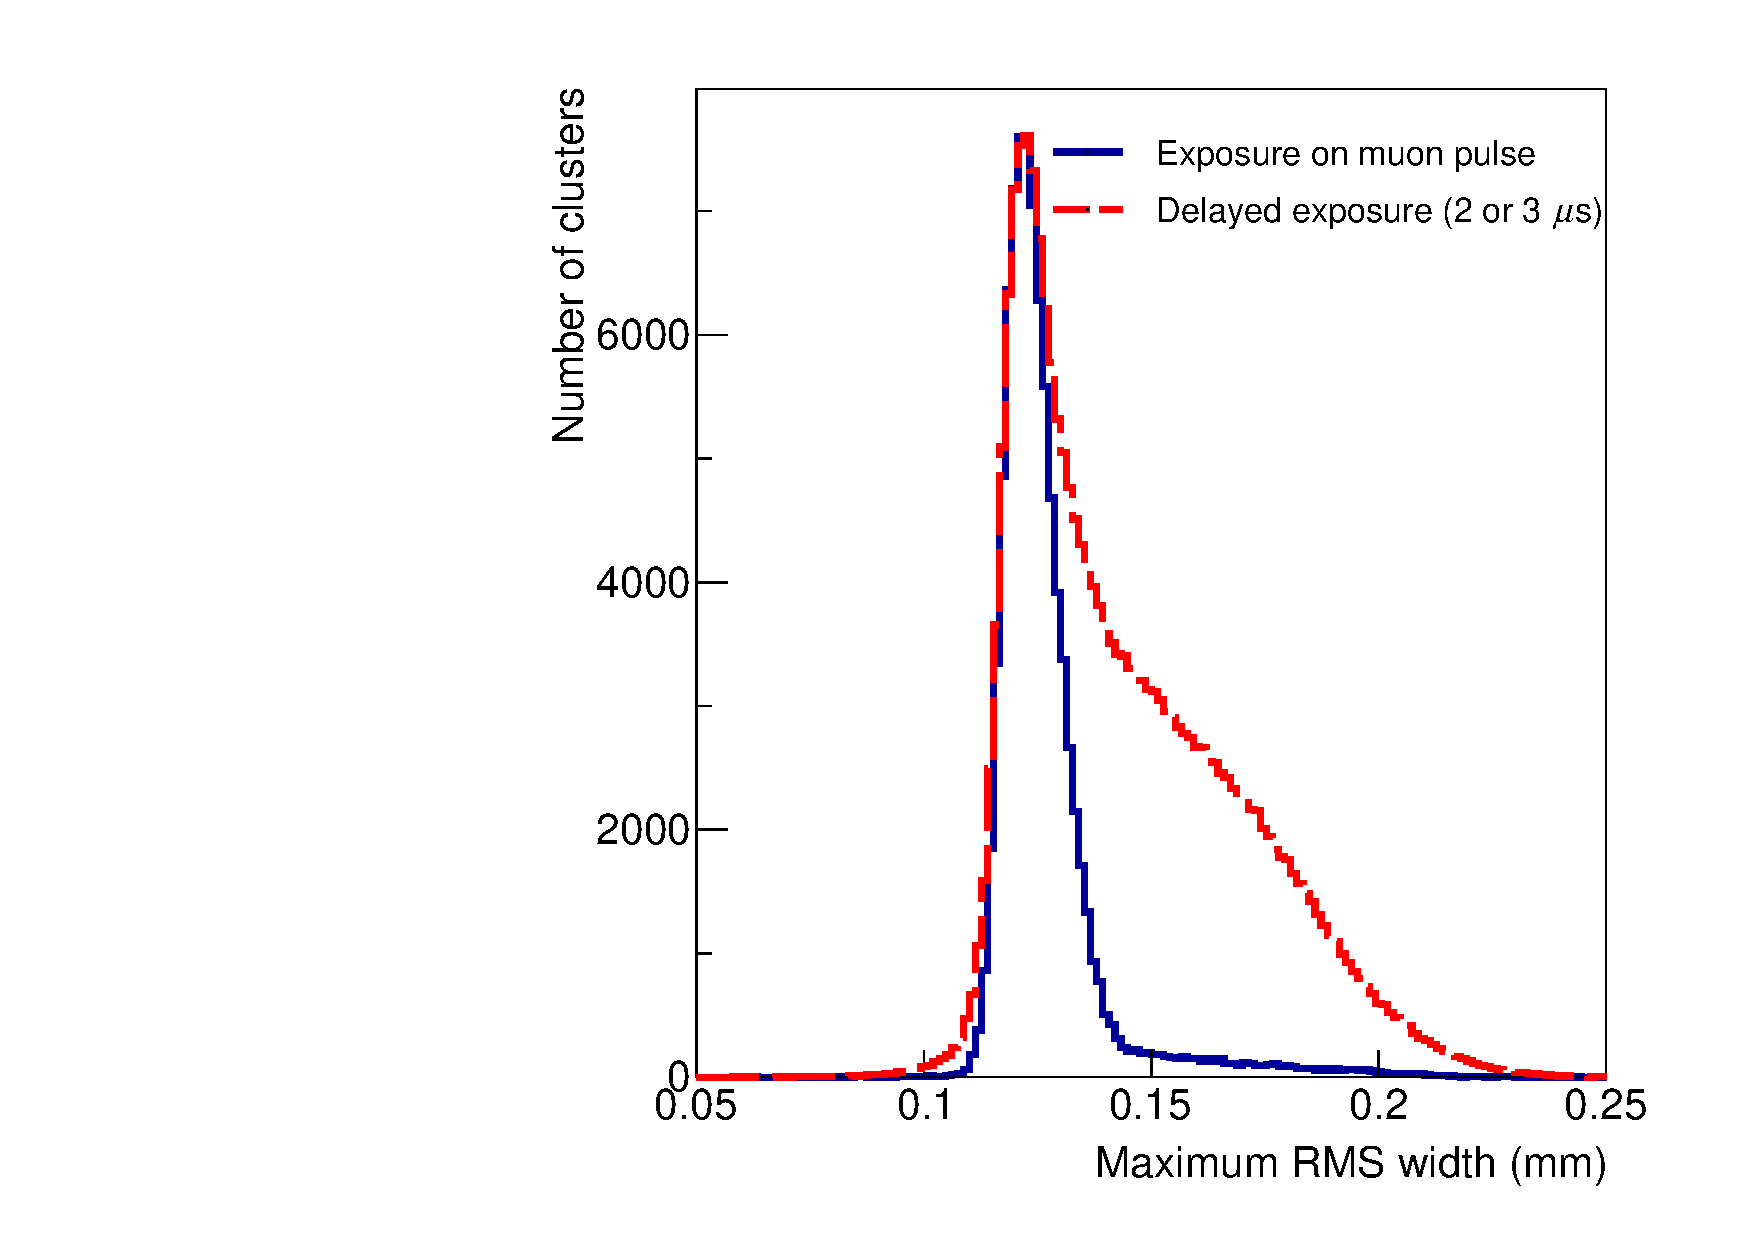
\includegraphics[width=\columnwidth]{figure/RMS_legend_v2.pdf}
	\caption{Signal's maximum RMS width histogram for the
          exposure on muon pulse (solid) and the delayed exposure
          (dashed) after rotating axes. The normalization is done for delayed exposure histogram by matching the peak height to that of exposure on muon pulse histogram.}
	\label{fig:positron_width}
\end{figure}

The time distribution of the decay positrons should be described
by an exponential decay function smeared by the time distribution
of the incoming muon beam.  In order to study the time distribution, data
were taken by changing the trigger timing from
$\SI{-0.5}{\micro\s}$ to $\SI{10}{\micro\s}$ with high intensity
% GMM Quantitatively, how high was the intensity?
muon beam. %The total ADC sum distribution versus the trigger time
%is shown in Fig.~\ref{fig:time_distribution}.

% GMM There has been no discussion of the time structure of the
% beam, especially the two pulse structre, the pulse separation,
% and the time width of each pulse. That becomes relevant in
% this analysis and should not be ignored.

For a $\SI{500}{\nano\s}$ exposure with $t_{delay} = \SI{0}{\micro\s}$, $\SI{11}{\percent}$ of the
stopped muons are expected to decay to the positrons within the
% GMM I would expect this number to be 20%. Could you please
% check? Or maybe I don't understand... shouldn't the fraction be
% (1. - exp(-(0.5/2.2)))?
exposure. The contribution of the decay positrons to the BPM
signal is deduced from the total ADC sum distribution in Fig. \ref{fig:time_distribution}. An exponential function with a constant background term is fitted to the data in the time region
later than $\SI{2}{\micro\s}$, in order to avoid the
contributions of incident muons. The measured decay parameter
$\tau_{\mu}=\SI{2.12 \pm 0.09}{\micro\s}$ agrees with the muon
% GMM Reference for muon lifetime?
lifetime \cite{muon_pdg}. The fraction of the positron contribution to the total
ADC sum, $\varepsilon$, is $\SI{2.51\pm0.17}{\percent}$.

The number of muons reaching the BPM has been estimated from the
total ADC sum. The necessary calibration has been obtained from
the analysis of low intensity muon beam data where the response
of each individual particle ($\mu^+$ or $e^+$) is identified. The
average ADC count generated by a single cluster, $a$, is obtained
by dividing the total ADC count by the number of detected
clusters in the CCD image. The overlapping events of clusters are assumed to be negligible considering the size of MCP active area and the cluster region.
% GMM Can you state what assumptions are made in this derivation,
% even if they are trivial?
% For example, no count rate effects such as dead time or
% saturation? Or is no such assumption necessary?

\begin{figure}[btp]
	\centering
	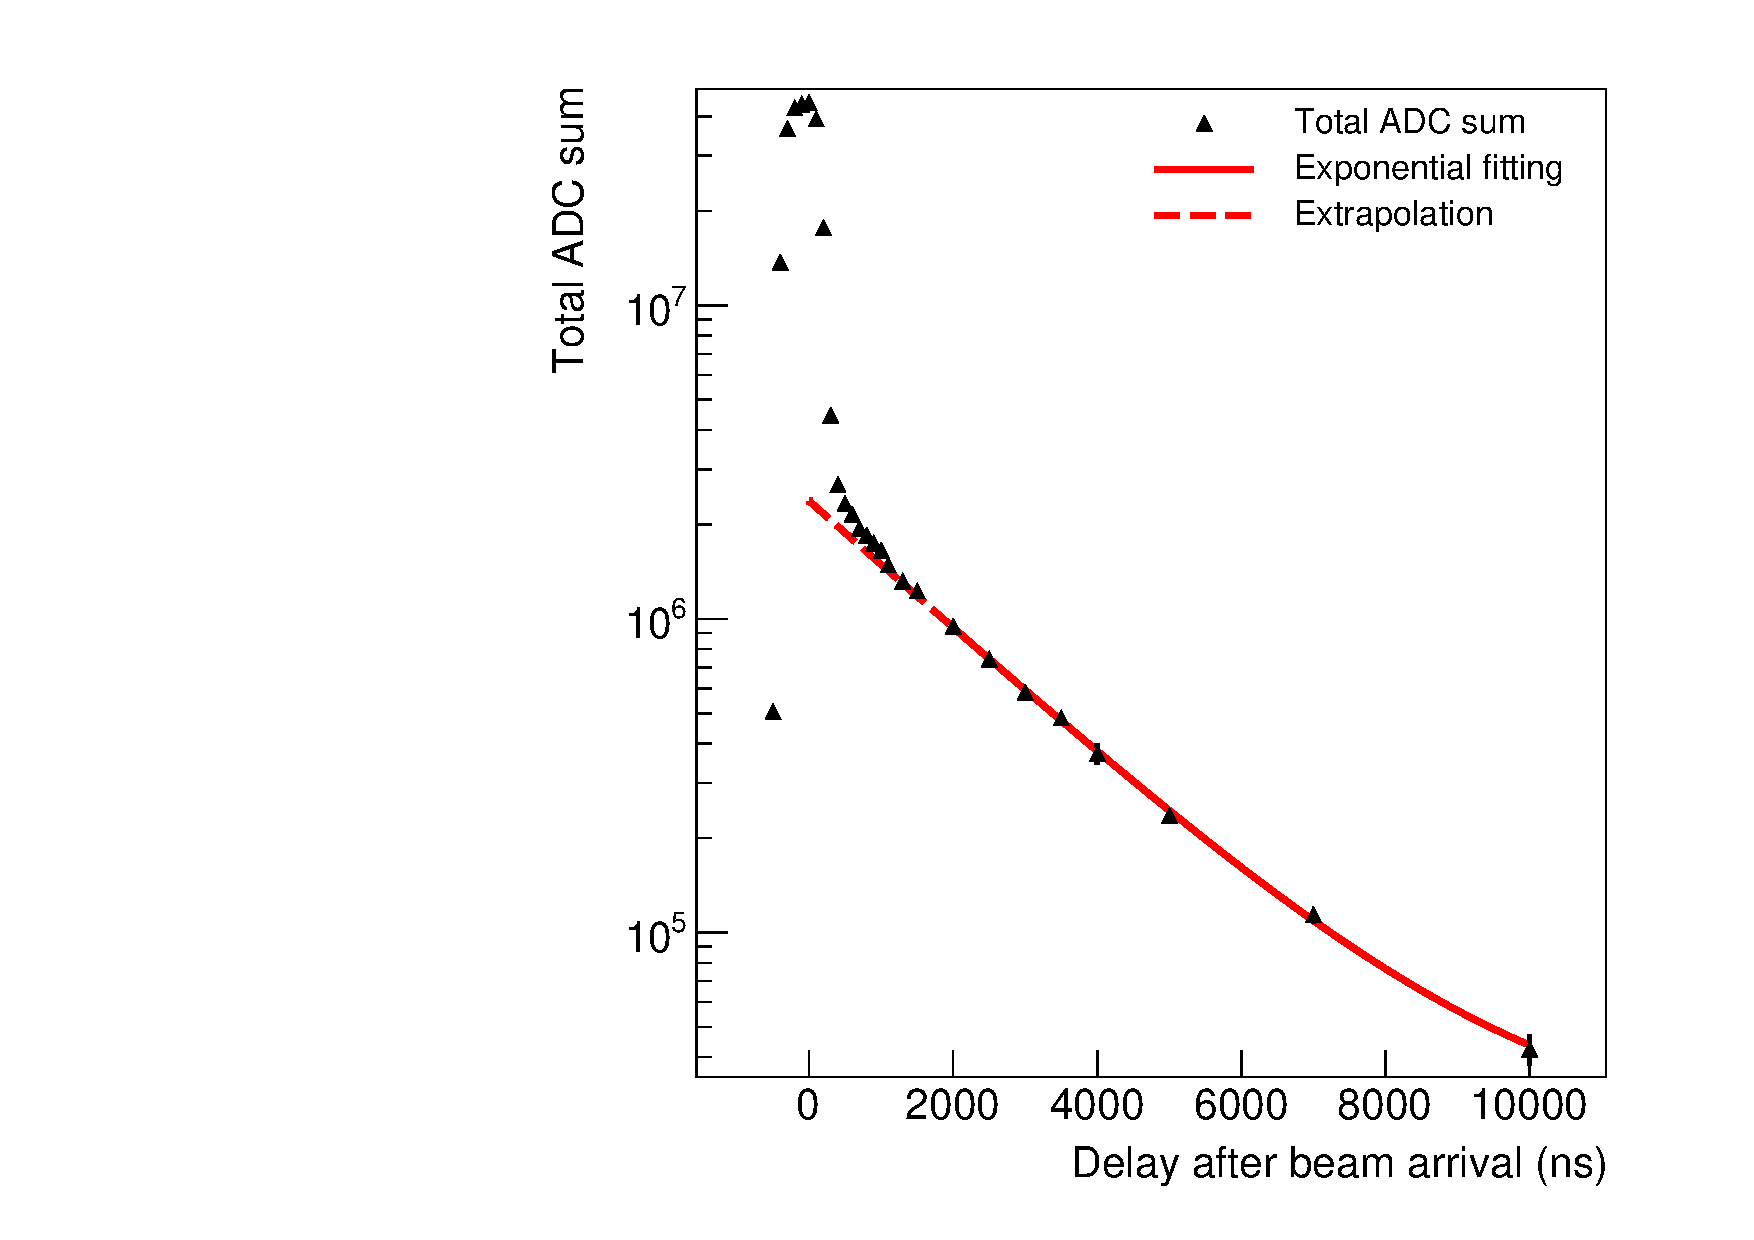
\includegraphics[width=\columnwidth]{figure/Decay_v3.pdf}
	\caption{The time distribution of BPM signal intensity
          with different trigger time. An exponential function with a constant background term is
          fitted from \SI{2000}{\ns} to \SI{10000}{\ns} and
          extrapolation to \SI{0}{\ns}, the exposure on the muon beam arrival time, is shown.}
	\label{fig:time_distribution}
\end{figure}
% GMM As mentioned above, what is t=0 for the extrapolation,
% especially with the muon beam time structure?

The parameter $a$ from the data in the muon arrival time window
is insufficient for the estimation of the number of muons because
it contains contributions of both muons and decay
positrons. On the other hand, the data taken after some delay
from muon arrival contain contributions primarily from decay
positrons. By applying cluster analysis to this delayed data, the average
ADC count generated by a single cluster of positron, $a_e$, is
obtained. For estimating the number of positron clusters out of
the total number of clusters, the $a_e$ value is used together
with $\varepsilon$, the measured ADC fraction of positron signal.

The total ADC sum in each picture for the exposure on the muon beam, $A$, is measured from data at
% GMM What pictures does this refer to? Do you mean exposures?
various muon beam intensities taken in the muon
beam time window.  The number of total clusters is calculated as $A/a$. In
this way, it is possible to obtain the number of total clusters
even when it is not possible to distinguish a single cluster due
to the high muon beam intensity.  On the other hand,
$\varepsilon A$ is considered as the ADC contribution from the
positrons. Thus, the number of clusters generated by the
positrons is also estimated as $\varepsilon A/a_e$. Then, the
rest of clusters are considered to be generated by muons. The
number of muon clusters $C_{\mu}$ is calculated with this
reasoning, {\it i.e}

\begin{linenomath}
\begin{equation}
C_{\mu} = C_{total} - C_{e}= A/a - A\varepsilon/a_e.
\end{equation}
\end{linenomath}

It is assumed that one muon generates only one cluster
since the transverse momentum of the muon is sufficiently limited
% Also by the short muon range? How far would a muon with similar
% energy but only transverse momentum? It might also be very small.
by the upstream collimator. Therefore, the calculated number of
muon clusters, $C_{\mu}$, is taken as the number of muons detected by the
BPM, $N_{\mu}$(BPM).%, shown in the vertical axis of
%Fig.~\ref{fig:muvsmu}.

An another independent estimation of the number of muons is made
from the number of positrons detected by the positron counter
located next to the BPM chamber. The proportionality constant has
been obtained from the simulation based on the actual
experimental setup implemented in the GEANT4 library
\cite{geant4}.  The simulation estimates the number of muons on
the MCP from the number of positrons detected by the positron
counter in coincidence with muons.

\begin{figure}[tbp]
	\centering
	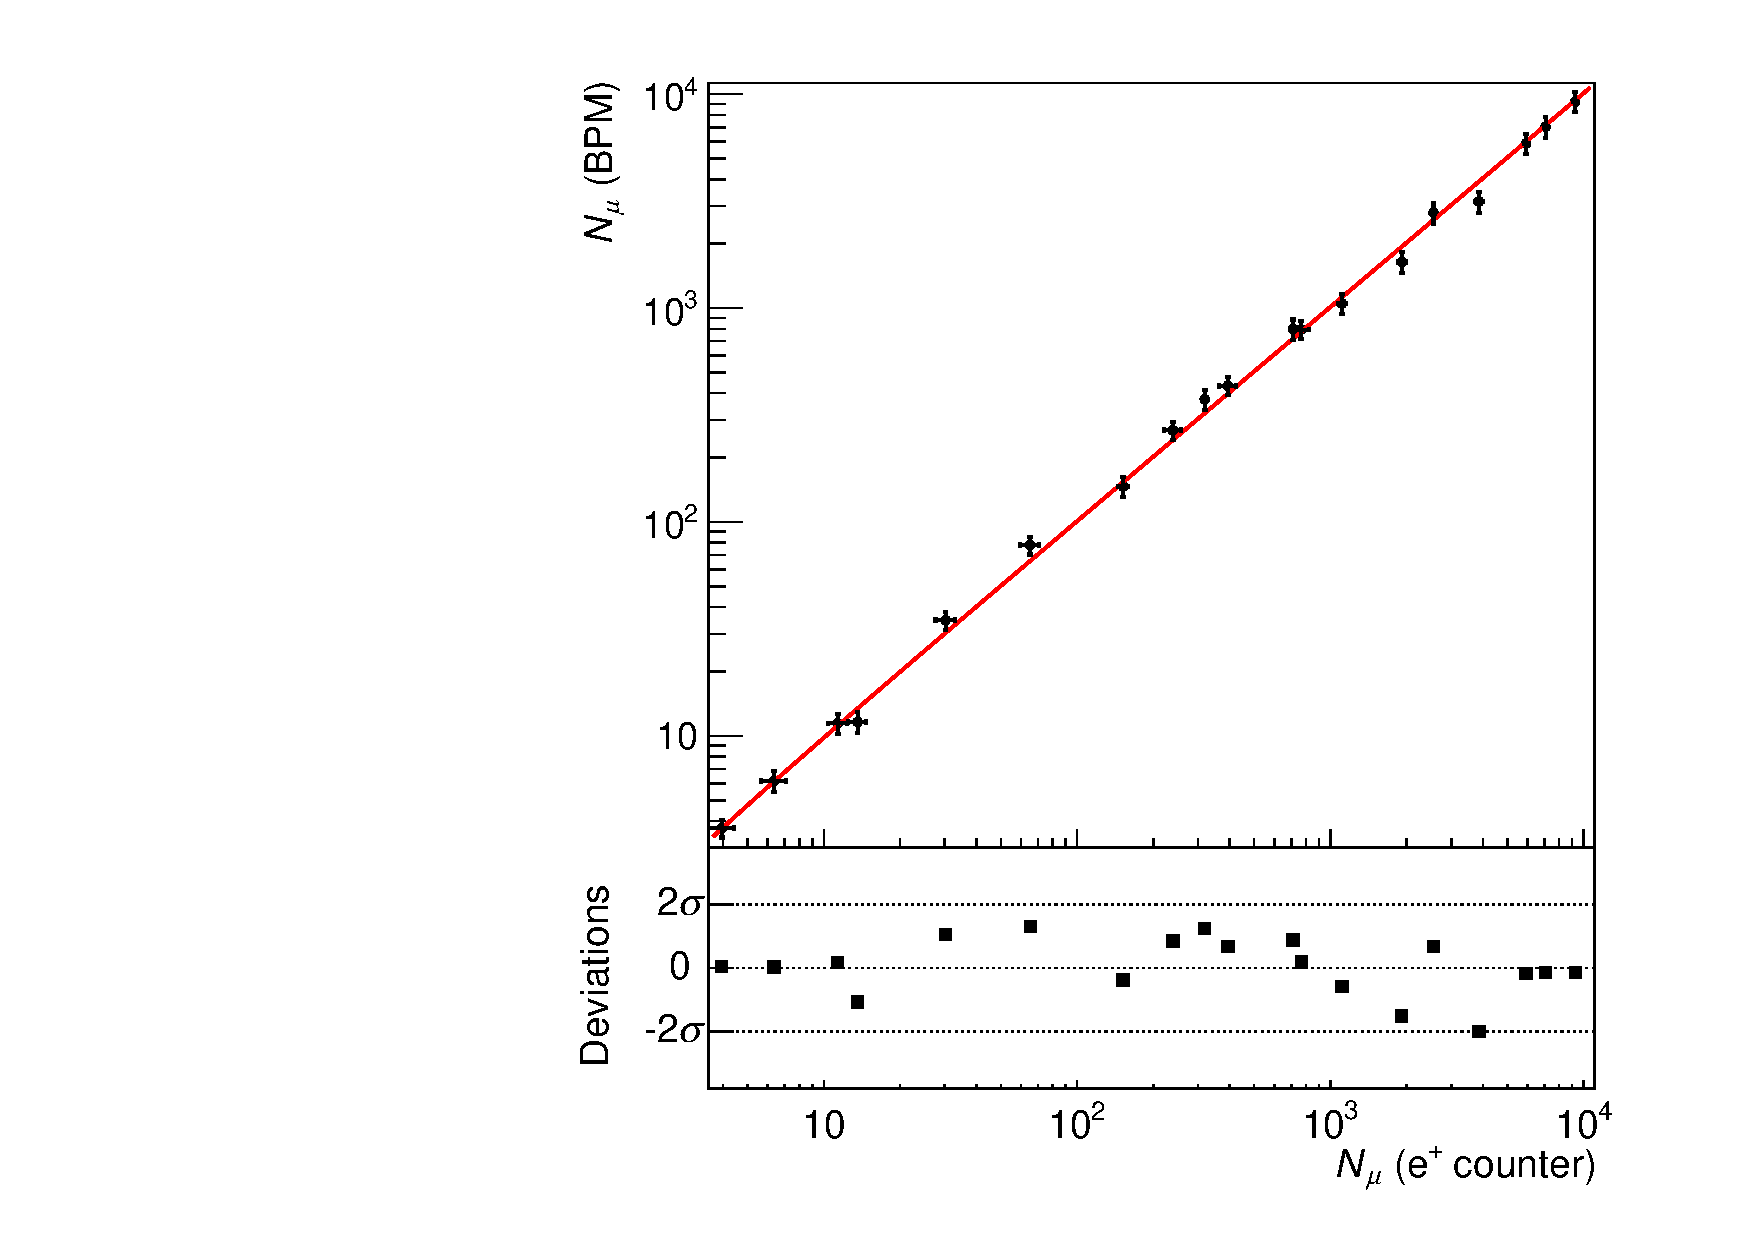
\includegraphics[width=\columnwidth]{figure/lin.pdf}
        \caption{Estimated number of muons from BPM vs estimated
          number of muons from positron counter. Both values are obtained for single pulse of the muon beam. Bottom graph
          shows residual distribution divided by error.}
\label{fig:muvsmu}
\end{figure}

The comparison of the number of muons obtained by these two
independent methods at various beam intensity is displayed on
Fig.~\ref{fig:muvsmu}. The detected muon beam intensity ranges
from a few muon to $10^{4}$ muon per bunch with three different
sizes of collimator hole and several settings of slits in the
beam line.

The statistical and systematic uncertainties are considered as
follows. The major systematic uncertainties are from
non-uniformity of gain (\SI{\sim 4.4}{\percent}), trigger timing
uncertainty (\SI{\sim 3.8}{\percent}), positron background
fitting (\SI{\sim 5.6}{\percent}) and inside light reflection
(\SI{\sim 2.4}{\percent}).  The statistical uncertainty is ten
times smaller than systematic uncertainties except for the low
intensity data where the statistical error is about
\SI{10}{\percent} for $N_\mu$($e^+$ counter).  The total error
is calculated as a quadratic sum of above uncertainties. It
ranges from \SI{9.6}{\percent} to \SI{11.2}{\percent} for 
$N_\mu$(BPM) and \SI{1.7}{\percent} to \SI{11.7}{\percent} for 
$N_\mu$($e^+$ counter).

A first order polynomial function is fitted to data.  Most
measurements agreed well with fitting function within $2\sigma$.
The fitted slope is \num{1.01 \pm 0.03}. No evidence of
saturation is observed.

\section{Spatial resolution}
 
The expected muon beam spot size during the first stages of muon
re-acceleration is a few millimeters.  Sharp-edge pictures were
taken with a collimator and UV light source to estimate the BPM
spatial resolution.  Usage of the UV light allows one to avoid
the positron background inevitably related to muons.

The half-circle open \SI{.5}{\cm} thick stainless collimator was
placed at \SI{1}{\cm} from the MCP front surface such that the
collimator's edge was near the MCP center.  The UV light provided
by the Xe-lamp source was guided by optical fibre to the
vacuum chamber.  The light guide output was centered with the main
MCP and collimator axis with distance along this axis about
% GMM Distance along this axis from the collimator? (to the light
% guide output)
%
%
% B.Kim : 15cm is longer than half of chamber length. I need to 
%         check but it would be distance from UV light feedthrough
%         to MCP. Do you have any information Gosha??
% G.Razuvaev : The full length of the chamber is 185 mm. The MCP is placed
%              at the centre, 185 mm / 2 = 92.5 mm. Then an 8" CF flange was
%              used, the flange thickness is 25 mm: 92.5 mm + 25 mm = 117.5 mm.
%              Then a flange with a UV guid input connected to the 8" CF
%              flange. I don't remember where was the output of this UF light
%              fibre. Then we should remember that the thickness of collimator
%              is 5 mm and it is placed in 10 mm from the MCP surface, that
%              means 117.5 mm - 5 mm - 10 mm = 102.5 mm. This is the best
%              estimation which I can do and 15 cm should be replaced by 10 cm.
\SI{10}{\cm}.  Thus the collimator casts a sharp shadow on the
MCP, and the image of the illuminated MCP surface produced a
% GMM I think this is what you mean by "plate".
signal to be analyzed for estimation of the spatial resolution.

The collimator edge image was aligned to pixel rows by picture
% GMM It is not clear what is meant by "picture rotation". Is the
% CCD that views the screen (and defines the pixel orientation)
% rotated? 
%
%
% S.Bae : As I understood, the picture rotation means that, not CCD itself, but
%         the image is rotated using ROOT.  That is because the straight edge of
%         the half circle collimator is not aligned with the x-axis of pixel but
%         slightly tilted.  By rotating the image, the axes are aligned and the
%         sliced histogram along y-axis, as in figure 8,  can be made in order
%         to check the resolution.
%
%
% G.Razuvaev : Sunghan, you are right.  The idea is to align the collimator
%              edge with pixels rows to make slicing easier.  This is made
%              offline when all pictures is taken.  Firstly it was dictaded by
%              the fact that we first take data and only several weeks/monthes
%              came to analysis.  The second reason is that it is not trivial to
%              alight so precisely the camera and collimator,  the scale of
%              desirable precision would be about the pixel size over the dia-
%              ter of the plate,  approximately 7.4 um / 40 mm ~= 0.02%.
rotation and one pixel thick vertical slices were obtained (see
Fig.~\ref{fig:half_circle}).  Discrete differentiation was
applied to each slice.  The peak, which corresponded to the
location of the collimator edge, was emphasized by Hann function
% GMM This is not a familiar term. Is there  a reference? Maybe
% use Gosha as below, if than explains it?
%
%
% B.Kim : Although there's no precise explanation about Hann windowing, We can find detail explanation in Gosha's paper.
%
%
% G.Razuvaev : As for me, I also hadn't met this term and function before the
%              this analysis, but it is one of the first solution to which
%              one come up when strat searching. The Hann function or hannging
%              is described in Wikipedia, it is part of the scipy and numpy
%              modules of python, it is included in R language, in Mathemati-
%              ca.
%              Yes, the function represented in the reference.  I think to
%              leave this as it is, if you don't mind.
multiplication.  The modulation transfer function was evaluated
by fast Fourier transformation.  The \SI{10}{\percent} height
frequency $\nu_{\SI{10}{\percent}}$ was obtained using a polynomial
approximation to additionally suppress statistical fluctuations.
More detailed information on the UV light resolution study is
found in Ref.~\cite{Gosha}.  $\nu_{\SI{10}{\percent}}$
corresponds to a spatial resolution of
$\Delta_\gamma = \SI{0.29}{\mm}$, which should be considered as
an upper limit due to light reflection from the edge's surface
induced by collimator and UV fiber misalignment.

\begin{figure}[tbp]
    \centering
	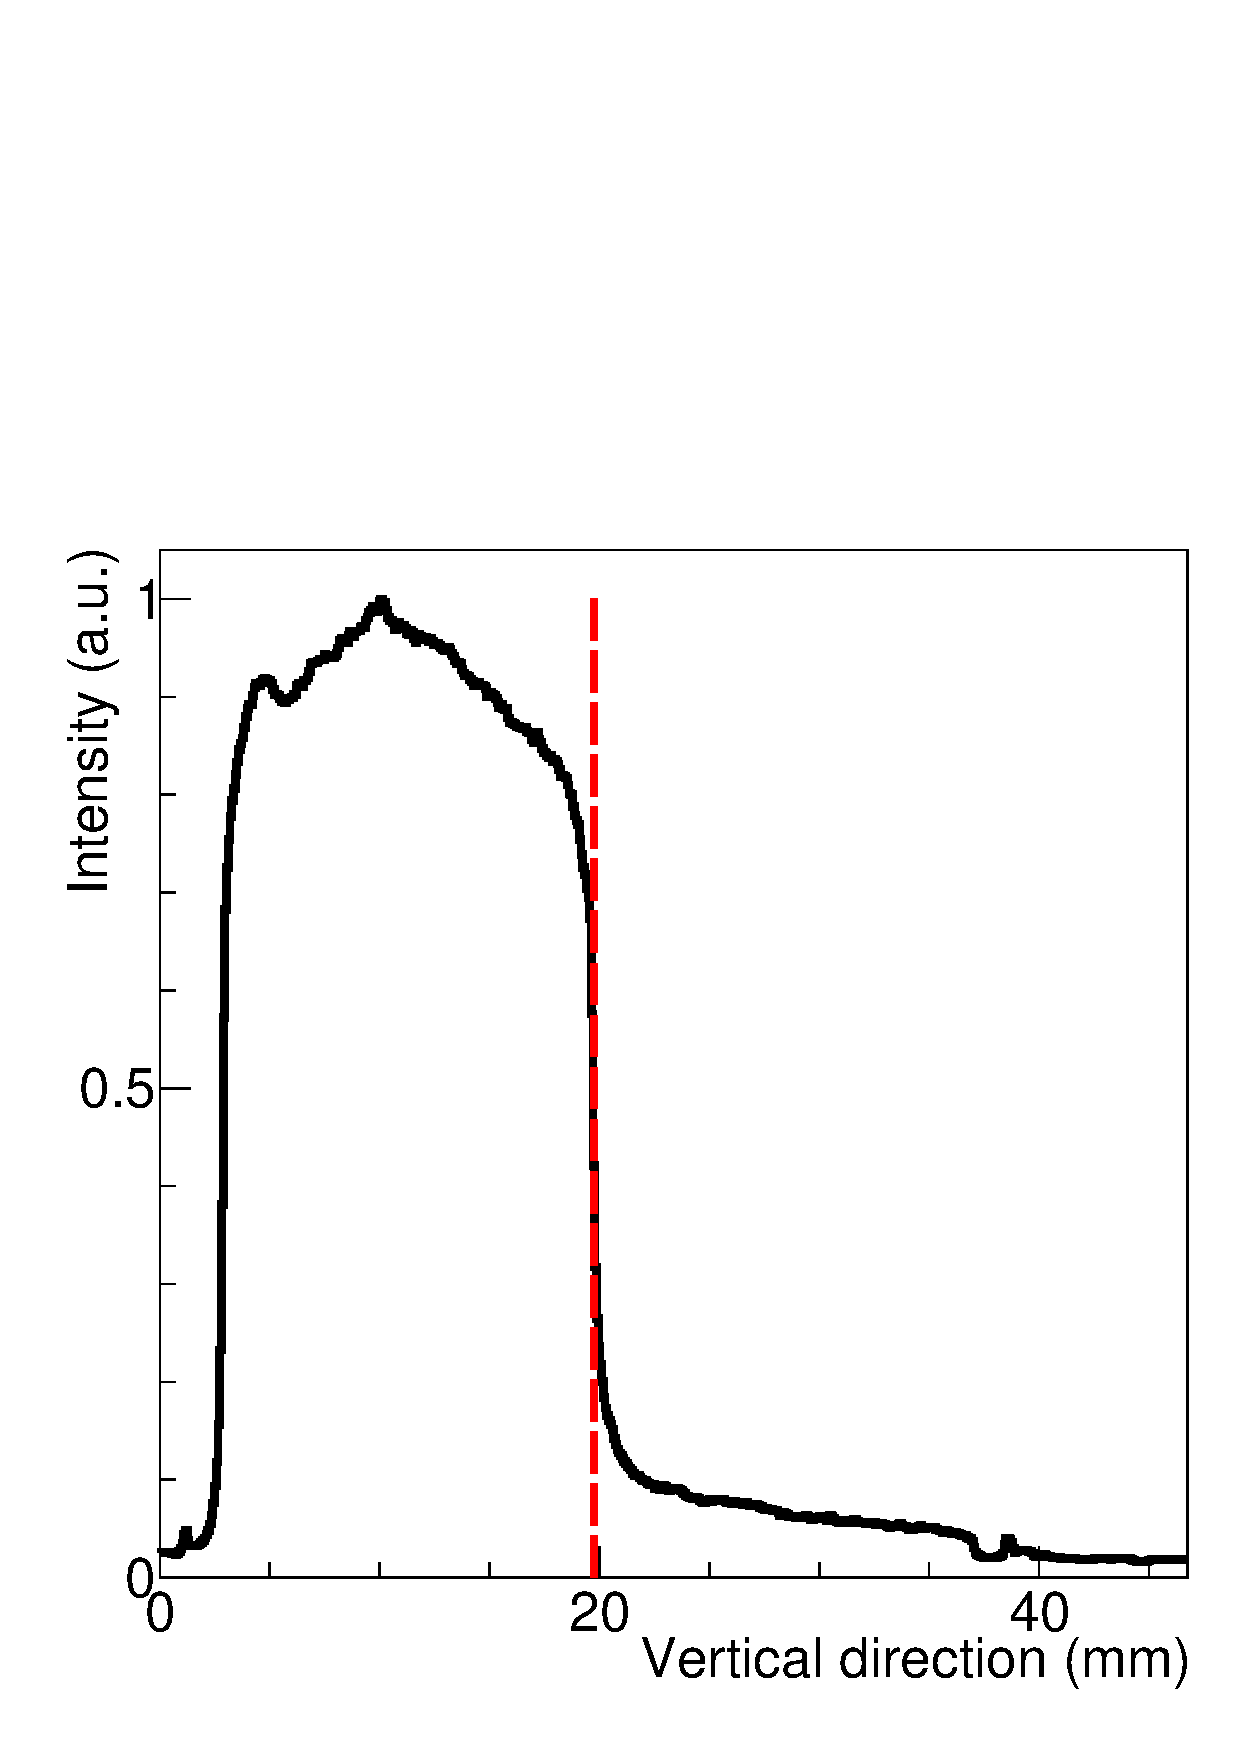
\includegraphics[width=\columnwidth]{figure/edge_image_w_uv_4_BH_axis.pdf}
	\caption{Projected ADC count distribution for UV light
          data on Y-axis following rotation to align the pixel
          orientation with the straight edge of the half circle
          collimator.}
% GMM Please check this caption and correct it if I have misunderstoond.
	\label{fig:half_circle}
\end{figure}

The spatial resolution upper limit for muons is considered to be
similar since the signal from single particles has almost
the same width:
$\Gamma_{\mu} / \Gamma_{\gamma} = \num{1.04 \pm 0.10}$.  Such a
resolution satisfies the accelerator requirements.

\section{Conclusions}

An MCP-based BPM has been developed to measure the profile of the
\iffalse ultracold\fi muon beam with low transeverse momentum for the J-PARC muon $g-2$/EDM experiment.
The BPM has been tested and evaluated by a surface muon beam and
also by a UV light source.  The spatial distribution of a muon
beam was measured with this
BPM with a high signal to background ratio between
muon and positron signals.  The positron background rate has been
reduced to a negligible level using a short exposure window for
the CCD camera and the additional selection of cluster
characteristics on the CCD image.  Good
linearity was confirmed without noticeable saturation from a few
muons to \num{e4} muons.  The spatial resolution was estimated as
less than \SI{.30}{\mm} from the UV light data.

\section*{Acknowledgment}

We are grateful to the J-PARC personnel for the excellent machine operation.
The experiment with muon beam was performed
at the Materials and Life Science Experimental Facility of the J-PARC 
under a user program (Proposal No. 2015A0321).
We thank Dr. T.\,U.~Ito for his advice on the technical design.
This work was supported by 
the JSPS KAKENHI Grant Numbers JP26287053, JP15H03666, JP16J07784,
the Korean National Research Foundation grants NRF-2015K2A2A4000092, NRF-2015H1A2A1030275, NRF-2015R1A4A1042542, NRF-2017R1A2B3007018,
the Russian Foundation for Basic Research grant RFBR 17-52-50064 and
the Russian Science Foundation grant RNF-17-12-01036,
Japan-Russia Research Cooperative Program.

\section*{References}

\bibliography{mybibfile}

\end{document}
